\begin{frame}
\frametitle{Visualising differences}
Neuroimagers like blobs and summary tables.

How do we best understand whole-brain multivariate differences?

Here's my attempt.....
\end{frame}


\begin{frame}
\frametitle{Exaggerated male brain}
\begin{center}
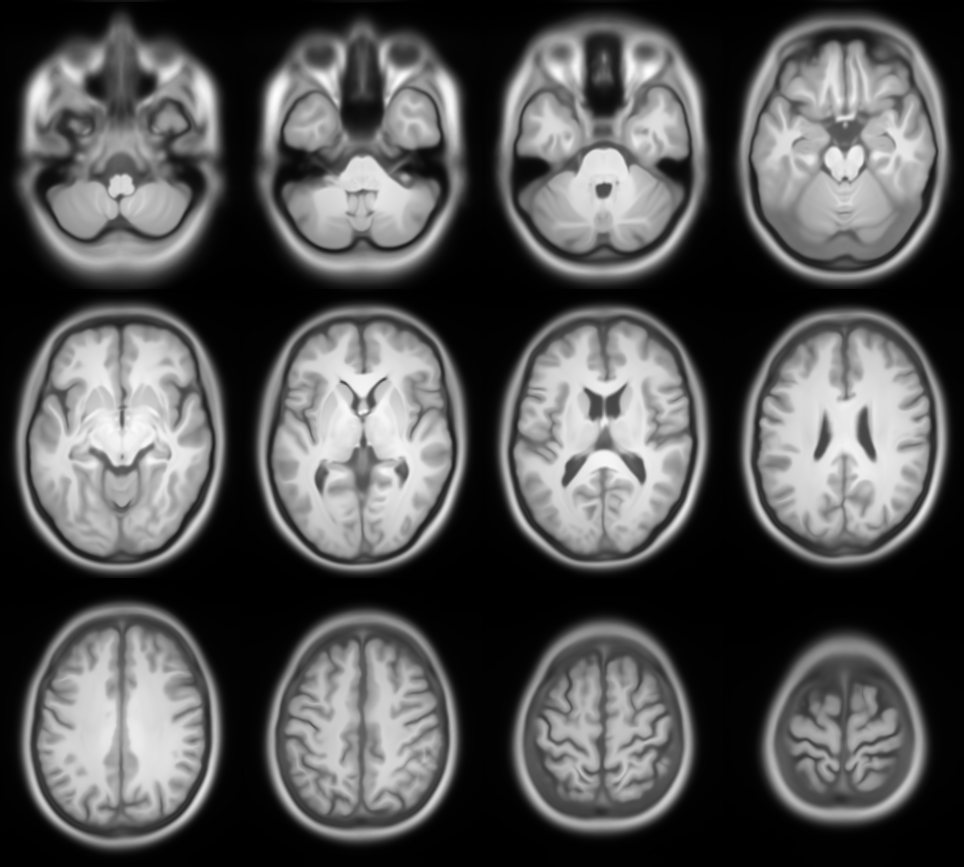
\includegraphics[width=.65\textwidth]{hyper_male}
\end{center}
\end{frame}



\begin{frame}
\frametitle{Average brain}
\begin{center}
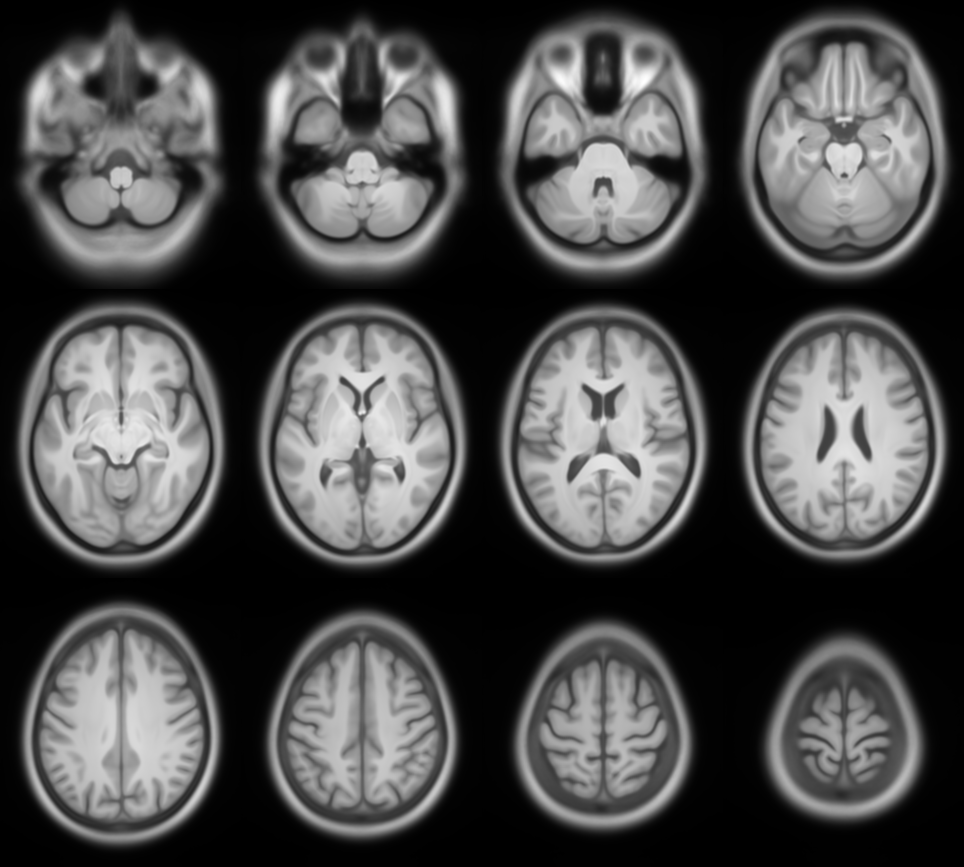
\includegraphics[width=.65\textwidth]{avgT1}
\end{center}
\end{frame}



\begin{frame}
\frametitle{Exaggerated female brain}
\begin{center}
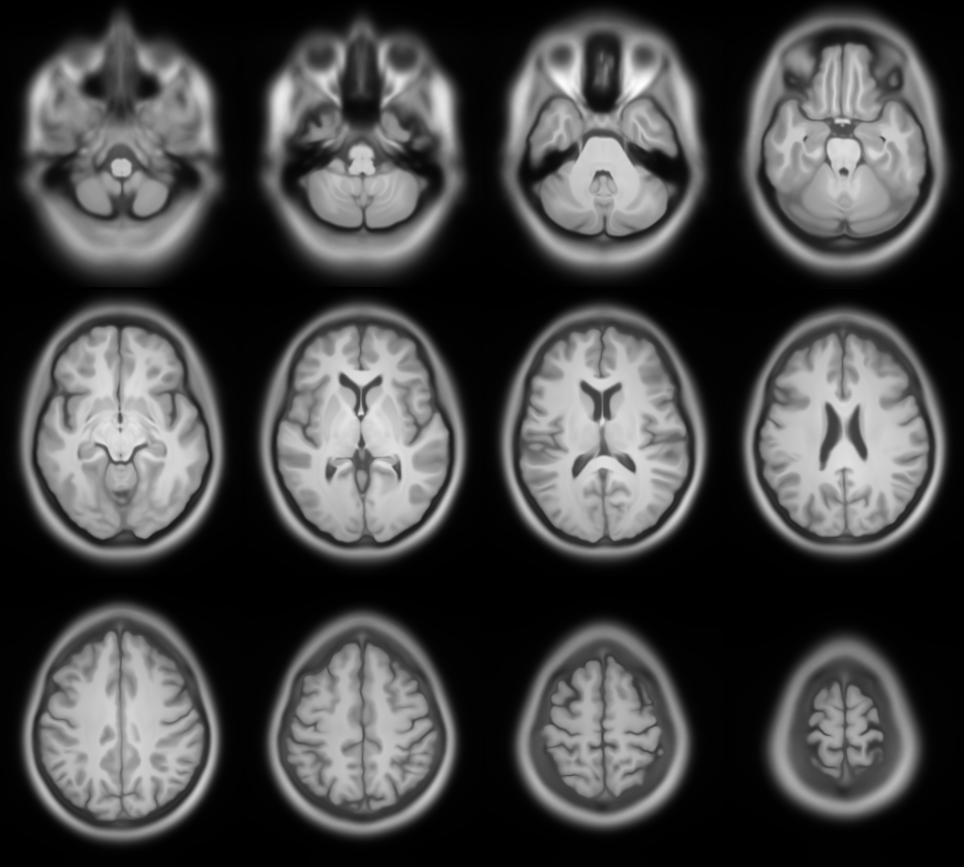
\includegraphics[width=.65\textwidth]{hyper_female}
\end{center}
\end{frame}


\begin{frame}
\frametitle{More information}
\begin{itemize}
\item These slides are available from\\
      \url{https://github.com/JohnAshburner/ISBI}
\item For more information, see\\
      Ashburner, John, and Stefan Kl\"oppel. ``Multivariate models of inter-subject anatomical variability.'' Neuroimage 56.2 (2011): 422-439.
\end{itemize}
\end{frame}
